% ==============================================================================
% PAGE 21: 6) ARDUINO NANO (Numbered Page 13)
% ==============================================================================
\subsubsection*{6) ARDUINO NANO}

\begin{center}
  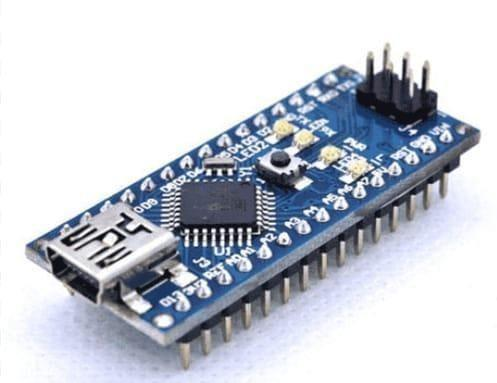
\includegraphics[width=65mm]{figures/fig6_arduino_nano.jpg}
\end{center}

\noindent
\begin{spacing}{1.2}
{\fontsize{10.2}{14.5}\selectfont
The Arduino Nano is a compact, microcontroller-based development board used as the main control unit in the solar tracking system of this project. It is responsible for processing the signals received from the Light Dependent Resistors (LDRs) and controlling the PMDC motor through the motor driver module, ensuring that the parabolic collector continuously follows the Sun's position throughout the day.\\[3.5mm]
\textbf{Function:}
\begin{itemize}[leftmargin=8mm, itemsep=2mm, label=\textbullet]
  \item Two LDR sensors are mounted on opposite sides of the collector.
  \item When sunlight intensity Differs between the two sensors, the Arduino Nano detects the voltage difference.
  \item It sends a control signal to the motor driver circuit, which activates the PMDC motor to rotate the collector toward the brighter side (toward the Sun).
  \item Once both LDRs sense equal light, the Arduino stops the motor --- meaning the collector is correctly aligned with the Sun.
\end{itemize}
}
\end{spacing}
\clearpage
